\documentclass{standalone}
\usepackage{tikz}
\usetikzlibrary{patterns, positioning}
\usepackage[sfdefault]{ClearSans} %% option 'sfdefault' activates Clear Sans as the default text font
\usepackage[T1]{fontenc}

\begin{document}
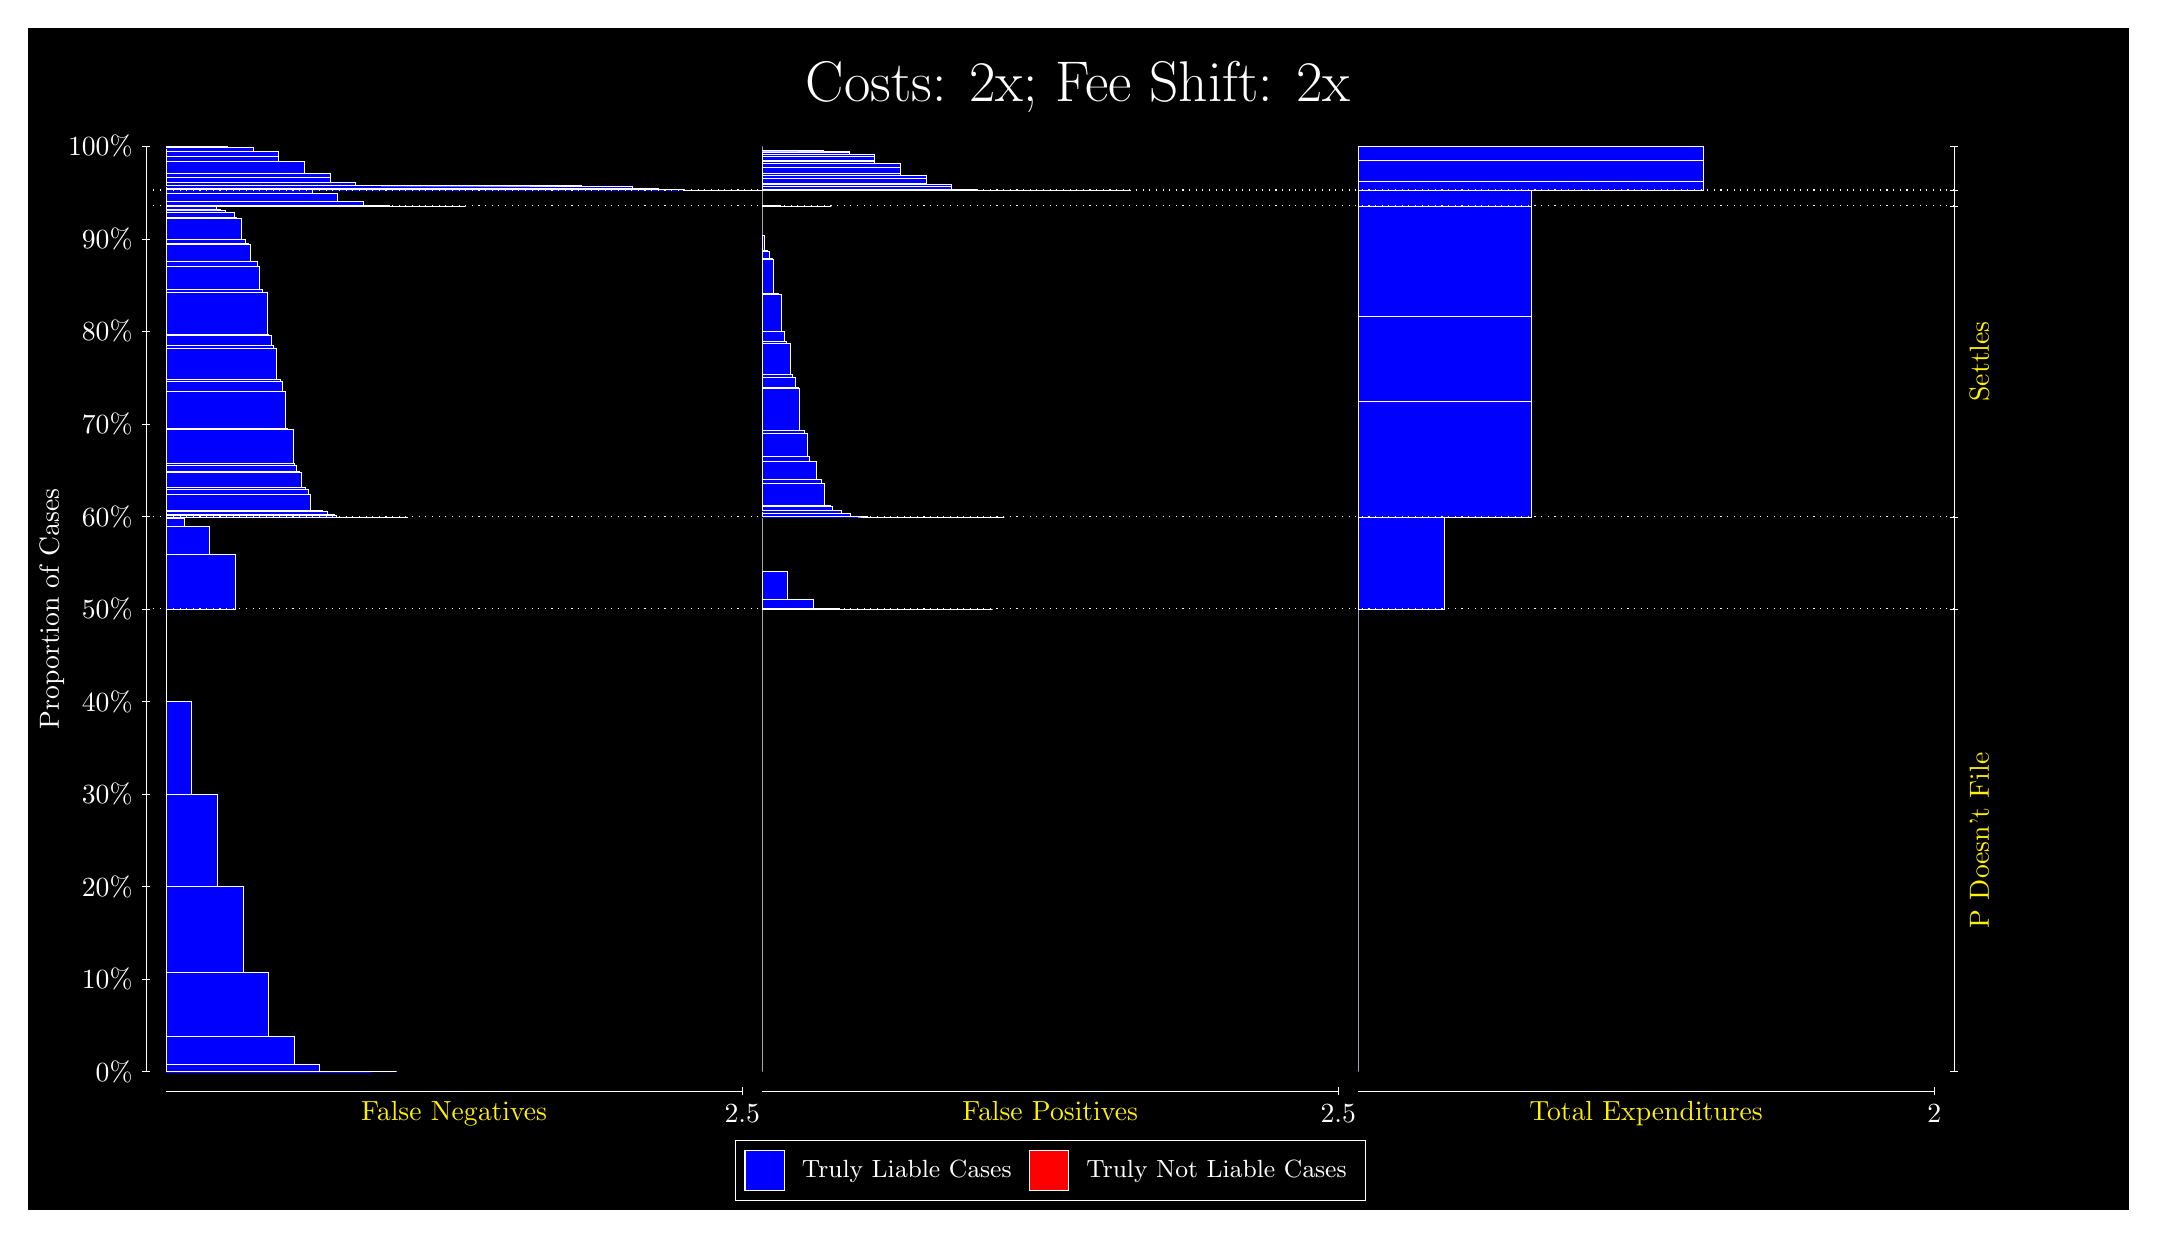
\begin{tikzpicture}
\draw[fill=black] (0,0) rectangle (26.667,15);
\draw[text=white] (0,13.5) rectangle (26.667,15) node[midway] {\huge Costs: 2x; Fee Shift: 2x};
\draw[white, very thin] (1.5,1.75) -- (1.5,13.5);
\node[rotate=90, text=white, anchor=center] at (0.3, 7.625) {Proportion of Cases};
\draw[white, very thin] (1.45,1.75) -- (1.55,1.75);
\node[text=white, anchor=east] at (1.45, 1.75) {0\%};
\draw[white, very thin] (1.45,2.925) -- (1.55,2.925);
\node[text=white, anchor=east] at (1.45, 2.925) {10\%};
\draw[white, very thin] (1.45,4.1) -- (1.55,4.1);
\node[text=white, anchor=east] at (1.45, 4.1) {20\%};
\draw[white, very thin] (1.45,5.275) -- (1.55,5.275);
\node[text=white, anchor=east] at (1.45, 5.275) {30\%};
\draw[white, very thin] (1.45,6.45) -- (1.55,6.45);
\node[text=white, anchor=east] at (1.45, 6.45) {40\%};
\draw[white, very thin] (1.45,7.625) -- (1.55,7.625);
\node[text=white, anchor=east] at (1.45, 7.625) {50\%};
\draw[white, very thin] (1.45,8.8) -- (1.55,8.8);
\node[text=white, anchor=east] at (1.45, 8.8) {60\%};
\draw[white, very thin] (1.45,9.975) -- (1.55,9.975);
\node[text=white, anchor=east] at (1.45, 9.975) {70\%};
\draw[white, very thin] (1.45,11.15) -- (1.55,11.15);
\node[text=white, anchor=east] at (1.45, 11.15) {80\%};
\draw[white, very thin] (1.45,12.325) -- (1.55,12.325);
\node[text=white, anchor=east] at (1.45, 12.325) {90\%};
\draw[white, very thin] (1.45,13.5) -- (1.55,13.5);
\node[text=white, anchor=east] at (1.45, 13.5) {100\%};

\draw[white, very thin] (24.457,1.75) -- (24.457,13.5);
\draw[white, very thin] (24.407,1.75) -- (24.507,1.75);
\node[anchor=west] at (24.407, 1.75) {};
\draw[white, very thin] (24.407,7.625) -- (24.507,7.625);
\node[anchor=west] at (24.407, 7.625) {};
\draw[white, very thin] (24.407,8.7932) -- (24.507,8.7932);
\node[anchor=west] at (24.407, 8.7932) {};
\draw[white, very thin] (24.407,12.744) -- (24.507,12.744);
\node[anchor=west] at (24.407, 12.744) {};
\draw[white, very thin] (24.407,12.945) -- (24.507,12.945);
\node[anchor=west] at (24.407, 12.945) {};
\draw[white, very thin] (24.407,13.5) -- (24.507,13.5);
\node[anchor=west] at (24.407, 13.5) {};

\draw[white, very thin, fill=blue] (1.75,1.75) rectangle (4.6775,1.75);
\draw[white, very thin, fill=blue] (1.75,1.75) rectangle (4.3523,1.7503);
\draw[white, very thin, fill=blue] (1.75,1.7503) rectangle (4.027,1.7576);
\draw[white, very thin, fill=blue] (1.75,1.7576) rectangle (3.7017,1.8362);
\draw[white, very thin, fill=blue] (1.75,1.8362) rectangle (3.3764,2.1987);
\draw[white, very thin, fill=blue] (1.75,2.1987) rectangle (3.0511,3.0112);
\draw[white, very thin, fill=blue] (1.75,3.0112) rectangle (2.7258,4.1076);
\draw[white, very thin, fill=blue] (1.75,4.1076) rectangle (2.4006,5.2753);
\draw[white, very thin, fill=blue] (1.75,5.2753) rectangle (2.0753,6.45);
\draw[white, very thin, fill=red] (1.75,6.45) rectangle (1.75,6.45);
\draw[white, very thin, fill=blue] (1.75,6.45) rectangle (1.75,7.625);
\draw[white, very thin, fill=blue] (1.75,7.625) rectangle (2.6283,8.3202);
\draw[white, very thin, fill=blue] (1.75,8.3202) rectangle (2.303,8.6767);
\draw[white, very thin, fill=blue] (1.75,8.6767) rectangle (1.9777,8.7787);
\draw[white, very thin, fill=red] (1.75,8.7787) rectangle (1.75,8.7787);
\draw[white, very thin, fill=blue] (1.75,8.7787) rectangle (1.75,8.7932);
\draw[white, very thin, fill=blue] (1.75,8.7932) rectangle (4.8239,8.7932);
\draw[white, very thin, fill=blue] (1.75,8.7932) rectangle (4.6775,8.7932);
\draw[white, very thin, fill=blue] (1.75,8.7932) rectangle (4.5312,8.7932);
\draw[white, very thin, fill=blue] (1.75,8.7932) rectangle (4.4986,8.7932);
\draw[white, very thin, fill=blue] (1.75,8.7932) rectangle (4.3848,8.7932);
\draw[white, very thin, fill=blue] (1.75,8.7932) rectangle (4.3523,8.7932);
\draw[white, very thin, fill=blue] (1.75,8.7932) rectangle (4.2384,8.794);
\draw[white, very thin, fill=blue] (1.75,8.794) rectangle (4.2059,8.7942);
\draw[white, very thin, fill=blue] (1.75,8.7942) rectangle (4.1734,8.7942);
\draw[white, very thin, fill=blue] (1.75,8.7942) rectangle (4.092,8.7943);
\draw[white, very thin, fill=blue] (1.75,8.7943) rectangle (4.0595,8.7945);
\draw[white, very thin, fill=blue] (1.75,8.7945) rectangle (4.027,8.7946);
\draw[white, very thin, fill=blue] (1.75,8.7946) rectangle (3.9457,8.7946);
\draw[white, very thin, fill=blue] (1.75,8.7946) rectangle (3.9131,8.8173);
\draw[white, very thin, fill=blue] (1.75,8.8173) rectangle (3.8806,8.8247);
\draw[white, very thin, fill=blue] (1.75,8.8247) rectangle (3.8481,8.8272);
\draw[white, very thin, fill=blue] (1.75,8.8272) rectangle (3.7993,8.8637);
\draw[white, very thin, fill=blue] (1.75,8.8637) rectangle (3.7668,8.8653);
\draw[white, very thin, fill=blue] (1.75,8.8653) rectangle (3.7342,8.8748);
\draw[white, very thin, fill=blue] (1.75,8.8748) rectangle (3.7017,8.8773);
\draw[white, very thin, fill=blue] (1.75,8.8773) rectangle (3.6204,8.8794);
\draw[white, very thin, fill=blue] (1.75,8.8794) rectangle (3.5878,9.0805);
\draw[white, very thin, fill=blue] (1.75,9.0805) rectangle (3.5553,9.1439);
\draw[white, very thin, fill=blue] (1.75,9.1439) rectangle (3.5228,9.1636);
\draw[white, very thin, fill=blue] (1.75,9.1636) rectangle (3.474,9.3621);
\draw[white, very thin, fill=blue] (1.75,9.3621) rectangle (3.4415,9.3765);
\draw[white, very thin, fill=blue] (1.75,9.3765) rectangle (3.4089,9.4551);
\draw[white, very thin, fill=blue] (1.75,9.4551) rectangle (3.3764,9.471);
\draw[white, very thin, fill=blue] (1.75,9.471) rectangle (3.3602,9.9037);
\draw[white, very thin, fill=blue] (1.75,9.9037) rectangle (3.2951,9.9225);
\draw[white, very thin, fill=blue] (1.75,9.9225) rectangle (3.2626,10.392);
\draw[white, very thin, fill=blue] (1.75,10.392) rectangle (3.23,10.513);
\draw[white, very thin, fill=blue] (1.75,10.513) rectangle (3.1975,10.542);
\draw[white, very thin, fill=blue] (1.75,10.542) rectangle (3.1487,10.939);
\draw[white, very thin, fill=blue] (1.75,10.939) rectangle (3.1162,10.967);
\draw[white, very thin, fill=blue] (1.75,10.967) rectangle (3.0837,11.097);
\draw[white, very thin, fill=blue] (1.75,11.097) rectangle (3.0511,11.113);
\draw[white, very thin, fill=blue] (1.75,11.113) rectangle (3.0349,11.645);
\draw[white, very thin, fill=blue] (1.75,11.645) rectangle (2.9698,11.682);
\draw[white, very thin, fill=blue] (1.75,11.682) rectangle (2.9373,11.978);
\draw[white, very thin, fill=blue] (1.75,11.978) rectangle (2.9048,12.034);
\draw[white, very thin, fill=blue] (1.75,12.034) rectangle (2.8722,12.042);
\draw[white, very thin, fill=blue] (1.75,12.042) rectangle (2.8234,12.261);
\draw[white, very thin, fill=blue] (1.75,12.261) rectangle (2.7909,12.271);
\draw[white, very thin, fill=blue] (1.75,12.271) rectangle (2.7584,12.316);
\draw[white, very thin, fill=blue] (1.75,12.316) rectangle (2.7258,12.319);
\draw[white, very thin, fill=blue] (1.75,12.319) rectangle (2.7096,12.592);
\draw[white, very thin, fill=blue] (1.75,12.592) rectangle (2.6445,12.605);
\draw[white, very thin, fill=blue] (1.75,12.605) rectangle (2.612,12.658);
\draw[white, very thin, fill=blue] (1.75,12.658) rectangle (2.5795,12.663);
\draw[white, very thin, fill=blue] (1.75,12.663) rectangle (2.5469,12.664);
\draw[white, very thin, fill=blue] (1.75,12.664) rectangle (2.4982,12.693);
\draw[white, very thin, fill=blue] (1.75,12.693) rectangle (2.4656,12.694);
\draw[white, very thin, fill=blue] (1.75,12.694) rectangle (2.4331,12.697);
\draw[white, very thin, fill=blue] (1.75,12.697) rectangle (2.4006,12.697);
\draw[white, very thin, fill=blue] (1.75,12.697) rectangle (2.3843,12.738);
\draw[white, very thin, fill=blue] (1.75,12.738) rectangle (2.3192,12.739);
\draw[white, very thin, fill=blue] (1.75,12.739) rectangle (2.2867,12.742);
\draw[white, very thin, fill=blue] (1.75,12.742) rectangle (2.2542,12.742);
\draw[white, very thin, fill=blue] (1.75,12.742) rectangle (2.2217,12.742);
\draw[white, very thin, fill=blue] (1.75,12.742) rectangle (2.1729,12.743);
\draw[white, very thin, fill=blue] (1.75,12.743) rectangle (2.1403,12.743);
\draw[white, very thin, fill=blue] (1.75,12.743) rectangle (2.1078,12.743);
\draw[white, very thin, fill=blue] (1.75,12.743) rectangle (2.0753,12.743);
\draw[white, very thin, fill=blue] (1.75,12.743) rectangle (2.059,12.744);
\draw[white, very thin, fill=blue] (1.75,12.744) rectangle (1.994,12.744);
\draw[white, very thin, fill=blue] (1.75,12.744) rectangle (1.9614,12.744);
\draw[white, very thin, fill=blue] (1.75,12.744) rectangle (1.9289,12.744);
\draw[white, very thin, fill=blue] (1.75,12.744) rectangle (1.8964,12.744);
\draw[white, very thin, fill=blue] (1.75,12.744) rectangle (1.8476,12.744);
\draw[white, very thin, fill=blue] (1.75,12.744) rectangle (1.8151,12.744);
\draw[white, very thin, fill=blue] (1.75,12.744) rectangle (1.7825,12.744);
\draw[white, very thin, fill=red] (1.75,12.744) rectangle (1.75,12.744);
\draw[white, very thin, fill=blue] (1.75,12.744) rectangle (1.75,12.744);
\draw[white, very thin, fill=blue] (1.75,12.744) rectangle (5.5558,12.744);
\draw[white, very thin, fill=blue] (1.75,12.744) rectangle (5.2305,12.744);
\draw[white, very thin, fill=blue] (1.75,12.744) rectangle (4.9052,12.744);
\draw[white, very thin, fill=blue] (1.75,12.744) rectangle (4.58,12.751);
\draw[white, very thin, fill=blue] (1.75,12.751) rectangle (4.2547,12.805);
\draw[white, very thin, fill=blue] (1.75,12.805) rectangle (3.9294,12.899);
\draw[white, very thin, fill=blue] (1.75,12.899) rectangle (3.6041,12.94);
\draw[white, very thin, fill=blue] (1.75,12.94) rectangle (3.2788,12.945);
\draw[white, very thin, fill=blue] (1.75,12.945) rectangle (2.9535,12.945);
\draw[white, very thin, fill=blue] (1.75,12.945) rectangle (2.6283,12.945);
\draw[white, very thin, fill=red] (1.75,12.945) rectangle (1.75,12.945);
\draw[white, very thin, fill=blue] (1.75,12.945) rectangle (9.9471,12.945);
\draw[white, very thin, fill=blue] (1.75,12.945) rectangle (9.6218,12.945);
\draw[white, very thin, fill=blue] (1.75,12.945) rectangle (9.2966,12.945);
\draw[white, very thin, fill=blue] (1.75,12.945) rectangle (8.9713,12.945);
\draw[white, very thin, fill=blue] (1.75,12.945) rectangle (8.9713,12.945);
\draw[white, very thin, fill=blue] (1.75,12.945) rectangle (8.646,12.946);
\draw[white, very thin, fill=blue] (1.75,12.946) rectangle (8.3207,12.95);
\draw[white, very thin, fill=blue] (1.75,12.95) rectangle (8.3207,12.951);
\draw[white, very thin, fill=blue] (1.75,12.951) rectangle (7.9954,12.961);
\draw[white, very thin, fill=blue] (1.75,12.961) rectangle (7.9954,12.968);
\draw[white, very thin, fill=blue] (1.75,12.968) rectangle (7.6702,12.991);
\draw[white, very thin, fill=blue] (1.75,12.991) rectangle (7.3449,12.997);
\draw[white, very thin, fill=blue] (1.75,12.997) rectangle (7.3449,12.998);
\draw[white, very thin, fill=blue] (1.75,12.998) rectangle (7.0196,12.999);
\draw[white, very thin, fill=blue] (1.75,12.999) rectangle (6.6943,12.999);
\draw[white, very thin, fill=blue] (1.75,12.999) rectangle (6.369,12.999);
\draw[white, very thin, fill=blue] (1.75,12.999) rectangle (6.369,12.999);
\draw[white, very thin, fill=blue] (1.75,12.999) rectangle (6.0437,12.999);
\draw[white, very thin, fill=blue] (1.75,12.999) rectangle (5.7835,12.999);
\draw[white, very thin, fill=blue] (1.75,12.999) rectangle (5.7185,12.999);
\draw[white, very thin, fill=blue] (1.75,12.999) rectangle (5.4582,12.999);
\draw[white, very thin, fill=blue] (1.75,12.999) rectangle (5.1329,12.999);
\draw[white, very thin, fill=blue] (1.75,12.999) rectangle (4.8077,12.999);
\draw[white, very thin, fill=blue] (1.75,12.999) rectangle (4.8077,12.999);
\draw[white, very thin, fill=blue] (1.75,12.999) rectangle (4.4824,13.001);
\draw[white, very thin, fill=blue] (1.75,13.001) rectangle (4.4824,13.004);
\draw[white, very thin, fill=blue] (1.75,13.004) rectangle (4.1571,13.045);
\draw[white, very thin, fill=blue] (1.75,13.045) rectangle (3.8318,13.103);
\draw[white, very thin, fill=blue] (1.75,13.103) rectangle (3.8318,13.16);
\draw[white, very thin, fill=blue] (1.75,13.16) rectangle (3.5065,13.311);
\draw[white, very thin, fill=blue] (1.75,13.311) rectangle (3.1812,13.369);
\draw[white, very thin, fill=blue] (1.75,13.369) rectangle (3.1812,13.372);
\draw[white, very thin, fill=blue] (1.75,13.372) rectangle (3.1812,13.431);
\draw[white, very thin, fill=blue] (1.75,13.431) rectangle (2.856,13.484);
\draw[white, very thin, fill=blue] (1.75,13.484) rectangle (2.856,13.485);
\draw[white, very thin, fill=blue] (1.75,13.485) rectangle (2.5307,13.49);
\draw[white, very thin, fill=blue] (1.75,13.49) rectangle (2.5307,13.49);
\draw[white, very thin, fill=blue] (1.75,13.49) rectangle (2.5307,13.498);
\draw[white, very thin, fill=blue] (1.75,13.498) rectangle (2.2054,13.5);
\draw[white, very thin, fill=blue] (1.75,13.5) rectangle (2.2054,13.5);
\draw[white, very thin, fill=blue] (1.75,13.5) rectangle (1.8801,13.5);
\draw[white, very thin, fill=blue] (1.75,13.5) rectangle (1.8801,13.5);
\draw[white, very thin, fill=red] (1.75,13.5) rectangle (1.75,13.5);
\draw[white, very thin, fill=blue] (1.75,13.5) rectangle (1.75,13.5);
\draw[white, very thin, fill=red] (9.3189,1.75) rectangle (9.3189,1.75);
\draw[white, very thin, fill=blue] (9.3189,1.75) rectangle (9.3189,7.625);
\draw[white, very thin, fill=red] (9.3189,7.625) rectangle (12.246,7.625);
\draw[white, very thin, fill=blue] (9.3189,7.625) rectangle (12.246,7.625);
\draw[white, very thin, fill=blue] (9.3189,7.625) rectangle (11.921,7.625);
\draw[white, very thin, fill=blue] (9.3189,7.625) rectangle (11.596,7.625);
\draw[white, very thin, fill=blue] (9.3189,7.625) rectangle (11.271,7.625);
\draw[white, very thin, fill=blue] (9.3189,7.625) rectangle (10.945,7.625);
\draw[white, very thin, fill=blue] (9.3189,7.625) rectangle (10.62,7.6257);
\draw[white, very thin, fill=blue] (9.3189,7.6257) rectangle (10.295,7.6395);
\draw[white, very thin, fill=blue] (9.3189,7.6395) rectangle (9.9694,7.7414);
\draw[white, very thin, fill=blue] (9.3189,7.7414) rectangle (9.6442,8.098);
\draw[white, very thin, fill=blue] (9.3189,8.098) rectangle (9.3189,8.7932);
\draw[white, very thin, fill=red] (9.3189,8.7932) rectangle (12.393,8.7932);
\draw[white, very thin, fill=blue] (9.3189,8.7932) rectangle (12.393,8.7932);
\draw[white, very thin, fill=blue] (9.3189,8.7932) rectangle (12.068,8.7932);
\draw[white, very thin, fill=red] (9.3189,8.7932) rectangle (11.954,8.7932);
\draw[white, very thin, fill=blue] (9.3189,8.7932) rectangle (11.954,8.7932);
\draw[white, very thin, fill=red] (9.3189,8.7932) rectangle (11.807,8.7932);
\draw[white, very thin, fill=blue] (9.3189,8.7932) rectangle (11.807,8.7932);
\draw[white, very thin, fill=blue] (9.3189,8.7932) rectangle (11.742,8.7932);
\draw[white, very thin, fill=red] (9.3189,8.7932) rectangle (11.661,8.7932);
\draw[white, very thin, fill=blue] (9.3189,8.7932) rectangle (11.661,8.7932);
\draw[white, very thin, fill=blue] (9.3189,8.7932) rectangle (11.628,8.7932);
\draw[white, very thin, fill=red] (9.3189,8.7932) rectangle (11.515,8.7932);
\draw[white, very thin, fill=blue] (9.3189,8.7932) rectangle (11.515,8.7932);
\draw[white, very thin, fill=blue] (9.3189,8.7932) rectangle (11.482,8.7932);
\draw[white, very thin, fill=blue] (9.3189,8.7932) rectangle (11.417,8.7932);
\draw[white, very thin, fill=red] (9.3189,8.7932) rectangle (11.368,8.7932);
\draw[white, very thin, fill=blue] (9.3189,8.7932) rectangle (11.368,8.7932);
\draw[white, very thin, fill=blue] (9.3189,8.7932) rectangle (11.336,8.7932);
\draw[white, very thin, fill=blue] (9.3189,8.7932) rectangle (11.303,8.7932);
\draw[white, very thin, fill=red] (9.3189,8.7932) rectangle (11.222,8.7932);
\draw[white, very thin, fill=blue] (9.3189,8.7932) rectangle (11.222,8.7932);
\draw[white, very thin, fill=blue] (9.3189,8.7932) rectangle (11.189,8.7932);
\draw[white, very thin, fill=blue] (9.3189,8.7932) rectangle (11.157,8.7932);
\draw[white, very thin, fill=blue] (9.3189,8.7932) rectangle (11.092,8.7932);
\draw[white, very thin, fill=red] (9.3189,8.7932) rectangle (11.075,8.7932);
\draw[white, very thin, fill=blue] (9.3189,8.7932) rectangle (11.075,8.7932);
\draw[white, very thin, fill=blue] (9.3189,8.7932) rectangle (11.043,8.7932);
\draw[white, very thin, fill=blue] (9.3189,8.7932) rectangle (11.01,8.7932);
\draw[white, very thin, fill=blue] (9.3189,8.7932) rectangle (10.978,8.7932);
\draw[white, very thin, fill=red] (9.3189,8.7932) rectangle (10.929,8.7932);
\draw[white, very thin, fill=blue] (9.3189,8.7932) rectangle (10.929,8.7932);
\draw[white, very thin, fill=blue] (9.3189,8.7932) rectangle (10.896,8.7932);
\draw[white, very thin, fill=blue] (9.3189,8.7932) rectangle (10.864,8.7932);
\draw[white, very thin, fill=blue] (9.3189,8.7932) rectangle (10.831,8.7932);
\draw[white, very thin, fill=blue] (9.3189,8.7932) rectangle (10.766,8.7947);
\draw[white, very thin, fill=blue] (9.3189,8.7947) rectangle (10.75,8.7947);
\draw[white, very thin, fill=blue] (9.3189,8.7947) rectangle (10.718,8.7947);
\draw[white, very thin, fill=blue] (9.3189,8.7947) rectangle (10.685,8.7948);
\draw[white, very thin, fill=blue] (9.3189,8.7948) rectangle (10.653,8.7956);
\draw[white, very thin, fill=blue] (9.3189,8.7956) rectangle (10.604,8.7956);
\draw[white, very thin, fill=blue] (9.3189,8.7956) rectangle (10.571,8.7958);
\draw[white, very thin, fill=blue] (9.3189,8.7958) rectangle (10.539,8.7983);
\draw[white, very thin, fill=blue] (9.3189,8.7983) rectangle (10.506,8.7991);
\draw[white, very thin, fill=blue] (9.3189,8.7991) rectangle (10.441,8.8401);
\draw[white, very thin, fill=blue] (9.3189,8.8401) rectangle (10.425,8.8402);
\draw[white, very thin, fill=blue] (9.3189,8.8402) rectangle (10.392,8.8436);
\draw[white, very thin, fill=blue] (9.3189,8.8436) rectangle (10.36,8.8442);
\draw[white, very thin, fill=blue] (9.3189,8.8442) rectangle (10.327,8.8734);
\draw[white, very thin, fill=blue] (9.3189,8.8734) rectangle (10.278,8.8739);
\draw[white, very thin, fill=blue] (9.3189,8.8739) rectangle (10.246,8.8798);
\draw[white, very thin, fill=blue] (9.3189,8.8798) rectangle (10.213,8.9324);
\draw[white, very thin, fill=blue] (9.3189,8.9324) rectangle (10.181,8.9453);
\draw[white, very thin, fill=blue] (9.3189,8.9453) rectangle (10.116,9.2186);
\draw[white, very thin, fill=blue] (9.3189,9.2186) rectangle (10.1,9.2211);
\draw[white, very thin, fill=blue] (9.3189,9.2211) rectangle (10.067,9.2668);
\draw[white, very thin, fill=blue] (9.3189,9.2668) rectangle (10.034,9.2767);
\draw[white, very thin, fill=blue] (9.3189,9.2767) rectangle (10.002,9.4954);
\draw[white, very thin, fill=blue] (9.3189,9.4954) rectangle (9.9532,9.5035);
\draw[white, very thin, fill=blue] (9.3189,9.5035) rectangle (9.9206,9.5593);
\draw[white, very thin, fill=blue] (9.3189,9.5593) rectangle (9.8881,9.8556);
\draw[white, very thin, fill=blue] (9.3189,9.8556) rectangle (9.8556,9.8922);
\draw[white, very thin, fill=blue] (9.3189,9.8922) rectangle (9.7905,10.424);
\draw[white, very thin, fill=blue] (9.3189,10.424) rectangle (9.7743,10.44);
\draw[white, very thin, fill=blue] (9.3189,10.44) rectangle (9.7417,10.571);
\draw[white, very thin, fill=blue] (9.3189,10.571) rectangle (9.7092,10.599);
\draw[white, very thin, fill=blue] (9.3189,10.599) rectangle (9.6767,10.996);
\draw[white, very thin, fill=blue] (9.3189,10.996) rectangle (9.6279,11.024);
\draw[white, very thin, fill=blue] (9.3189,11.024) rectangle (9.5954,11.145);
\draw[white, very thin, fill=blue] (9.3189,11.145) rectangle (9.5628,11.615);
\draw[white, very thin, fill=blue] (9.3189,11.615) rectangle (9.5303,11.634);
\draw[white, very thin, fill=blue] (9.3189,11.634) rectangle (9.4652,12.066);
\draw[white, very thin, fill=blue] (9.3189,12.066) rectangle (9.449,12.082);
\draw[white, very thin, fill=blue] (9.3189,12.082) rectangle (9.4165,12.161);
\draw[white, very thin, fill=blue] (9.3189,12.161) rectangle (9.3839,12.175);
\draw[white, very thin, fill=blue] (9.3189,12.175) rectangle (9.3514,12.374);
\draw[white, very thin, fill=blue] (9.3189,12.374) rectangle (9.3189,12.744);
\draw[white, very thin, fill=red] (9.3189,12.744) rectangle (10.197,12.744);
\draw[white, very thin, fill=blue] (9.3189,12.744) rectangle (10.197,12.744);
\draw[white, very thin, fill=blue] (9.3189,12.744) rectangle (9.8718,12.744);
\draw[white, very thin, fill=blue] (9.3189,12.744) rectangle (9.5466,12.75);
\draw[white, very thin, fill=blue] (9.3189,12.75) rectangle (9.3189,12.945);
\draw[white, very thin, fill=red] (9.3189,12.945) rectangle (14.003,12.945);
\draw[white, very thin, fill=blue] (9.3189,12.945) rectangle (14.003,12.945);
\draw[white, very thin, fill=red] (9.3189,12.945) rectangle (13.678,12.945);
\draw[white, very thin, fill=blue] (9.3189,12.945) rectangle (13.678,12.945);
\draw[white, very thin, fill=red] (9.3189,12.945) rectangle (13.352,12.945);
\draw[white, very thin, fill=blue] (9.3189,12.945) rectangle (13.352,12.945);
\draw[white, very thin, fill=blue] (9.3189,12.945) rectangle (13.027,12.945);
\draw[white, very thin, fill=red] (9.3189,12.945) rectangle (13.027,12.945);
\draw[white, very thin, fill=blue] (9.3189,12.945) rectangle (13.027,12.945);
\draw[white, very thin, fill=blue] (9.3189,12.945) rectangle (12.702,12.946);
\draw[white, very thin, fill=red] (9.3189,12.946) rectangle (12.702,12.946);
\draw[white, very thin, fill=blue] (9.3189,12.946) rectangle (12.702,12.946);
\draw[white, very thin, fill=blue] (9.3189,12.946) rectangle (12.377,12.947);
\draw[white, very thin, fill=red] (9.3189,12.947) rectangle (12.377,12.947);
\draw[white, very thin, fill=blue] (9.3189,12.947) rectangle (12.377,12.947);
\draw[white, very thin, fill=blue] (9.3189,12.947) rectangle (12.051,12.952);
\draw[white, very thin, fill=red] (9.3189,12.952) rectangle (12.051,12.952);
\draw[white, very thin, fill=blue] (9.3189,12.952) rectangle (12.051,12.96);
\draw[white, very thin, fill=blue] (9.3189,12.96) rectangle (12.051,12.96);
\draw[white, very thin, fill=blue] (9.3189,12.96) rectangle (12.051,12.96);
\draw[white, very thin, fill=blue] (9.3189,12.96) rectangle (11.726,12.992);
\draw[white, very thin, fill=red] (9.3189,12.992) rectangle (11.726,12.992);
\draw[white, very thin, fill=blue] (9.3189,12.992) rectangle (11.726,13.015);
\draw[white, very thin, fill=blue] (9.3189,13.015) rectangle (11.726,13.015);
\draw[white, very thin, fill=blue] (9.3189,13.015) rectangle (11.401,13.03);
\draw[white, very thin, fill=blue] (9.3189,13.03) rectangle (11.401,13.091);
\draw[white, very thin, fill=blue] (9.3189,13.091) rectangle (11.401,13.134);
\draw[white, very thin, fill=blue] (9.3189,13.134) rectangle (11.075,13.161);
\draw[white, very thin, fill=blue] (9.3189,13.161) rectangle (11.075,13.236);
\draw[white, very thin, fill=blue] (9.3189,13.236) rectangle (11.075,13.285);
\draw[white, very thin, fill=blue] (9.3189,13.285) rectangle (10.75,13.315);
\draw[white, very thin, fill=blue] (9.3189,13.315) rectangle (10.75,13.317);
\draw[white, very thin, fill=blue] (9.3189,13.317) rectangle (10.75,13.378);
\draw[white, very thin, fill=blue] (9.3189,13.378) rectangle (10.75,13.4);
\draw[white, very thin, fill=blue] (9.3189,13.4) rectangle (10.425,13.419);
\draw[white, very thin, fill=blue] (9.3189,13.419) rectangle (10.425,13.441);
\draw[white, very thin, fill=blue] (9.3189,13.441) rectangle (10.1,13.442);
\draw[white, very thin, fill=blue] (9.3189,13.442) rectangle (10.1,13.446);
\draw[white, very thin, fill=blue] (9.3189,13.446) rectangle (10.1,13.446);
\draw[white, very thin, fill=blue] (9.3189,13.446) rectangle (9.7743,13.446);
\draw[white, very thin, fill=blue] (9.3189,13.446) rectangle (9.7743,13.447);
\draw[white, very thin, fill=blue] (9.3189,13.447) rectangle (9.449,13.447);
\draw[white, very thin, fill=blue] (9.3189,13.447) rectangle (9.449,13.447);
\draw[white, very thin, fill=blue] (9.3189,13.447) rectangle (9.449,13.447);
\draw[white, very thin, fill=red] (9.3189,13.447) rectangle (9.3189,13.447);
\draw[white, very thin, fill=blue] (9.3189,13.447) rectangle (9.3189,13.5);
\draw[white, very thin, fill=red] (16.888,1.75) rectangle (16.888,1.75);
\draw[white, very thin, fill=blue] (16.888,1.75) rectangle (16.888,7.625);
\draw[white, very thin, fill=red] (16.888,7.625) rectangle (17.986,7.625);
\draw[white, very thin, fill=blue] (16.888,7.625) rectangle (17.986,8.7932);
\draw[white, very thin, fill=red] (16.888,8.7932) rectangle (19.083,8.7932);
\draw[white, very thin, fill=blue] (16.888,8.7932) rectangle (19.083,10.259);
\draw[white, very thin, fill=red] (16.888,10.259) rectangle (19.083,10.259);
\draw[white, very thin, fill=blue] (16.888,10.259) rectangle (19.083,11.342);
\draw[white, very thin, fill=red] (16.888,11.342) rectangle (19.083,11.342);
\draw[white, very thin, fill=blue] (16.888,11.342) rectangle (19.083,12.744);
\draw[white, very thin, fill=red] (16.888,12.744) rectangle (19.083,12.744);
\draw[white, very thin, fill=blue] (16.888,12.744) rectangle (19.083,12.945);
\draw[white, very thin, fill=red] (16.888,12.945) rectangle (21.279,12.945);
\draw[white, very thin, fill=blue] (16.888,12.945) rectangle (21.279,13.062);
\draw[white, very thin, fill=red] (16.888,13.062) rectangle (21.279,13.062);
\draw[white, very thin, fill=blue] (16.888,13.062) rectangle (21.279,13.317);
\draw[white, very thin, fill=red] (16.888,13.317) rectangle (21.279,13.317);
\draw[white, very thin, fill=blue] (16.888,13.317) rectangle (21.279,13.5);
\draw[white, dotted] (1.5,7.625) -- (24.457,7.625);
\draw[white, dotted] (1.5,8.7932) -- (24.457,8.7932);
\draw[white, dotted] (1.5,12.744) -- (24.457,12.744);
\draw[white, dotted] (1.5,12.945) -- (24.457,12.945);
\draw[white, very thin] (1.75,1.5) -- (9.0689,1.5);
\node[text=yellow, anchor=north] at (5.4094, 1.5) {False Negatives};
\draw[white, very thin] (9.0689,1.45) -- (9.0689,1.55);
\node[text=white, anchor=north] at (9.0689, 1.45) {2.5};

\draw[white, very thin] (9.3189,1.5) -- (16.638,1.5);
\node[text=yellow, anchor=north] at (12.978, 1.5) {False Positives};
\draw[white, very thin] (16.638,1.45) -- (16.638,1.55);
\node[text=white, anchor=north] at (16.638, 1.45) {2.5};

\draw[white, very thin] (16.888,1.5) -- (24.207,1.5);
\node[text=yellow, anchor=north] at (20.547, 1.5) {Total Expenditures};
\draw[white, very thin] (24.207,1.45) -- (24.207,1.55);
\node[text=white, anchor=north] at (24.207, 1.45) {2};

\node[text=yellow, centered, rotate=90] at (24.777, 4.6875) {P Doesn't File};

\node[text=yellow, centered, rotate=90] at (24.777, 10.769) {Settles};



\draw (12.978300999999998,1.5) node[draw=none] (baseCoordinate) {};
\begin{scope}[align=center]
        \matrix[scale=0.5, draw=white, below=0.5cm of baseCoordinate, nodes={draw}, column sep=0.1cm]{
            \node[rectangle, draw, minimum width=0.5cm, minimum height=0.5cm, fill=blue] {}; &
            \node[draw=none, font=\small, text=white] (B) {Truly Liable Cases}; &
            \node[rectangle, draw, minimum width=0.5cm, minimum height=0.5cm, fill=red] {}; &
            \node[draw=none, font=\small, text=white] (B) {Truly Not Liable Cases}; \\
            };
\end{scope}

\end{tikzpicture}
\end{document}